\documentclass[a4paper] {article}
\usepackage[utf8]{inputenc}
\usepackage{graphicx}

\title {Optimization and Parallelization \\ of the N-Body Simulation}
\author {Peter Boström \\ pbos@kth.se}

\begin {document}
\maketitle

\tableofcontents
\clearpage

\section{Introduction}

The N-body simulation is a simulation of gravitational forces between bodies. Every body is affected by every other body. This report aims to show that the simulation can be optimized significantly from its naive or simple solution. It also aims to investigate how well the n-body simulation can be parallelized. These simulations were done in three dimensions, but the problem is very similar regardless. There are possibly less issues of bodies clumping together when all bodies are distributed across more dimensions. It will unfortunately also show how overextensive mutex locking can break the performance of a program.

\section{Programs}

All programs are divided into two steps, first calculating forces per-body and then applying acceleration as well as velocity. All programs are implemented in C with the Pthreads library using a shared-memory programming model. All programs have a graphical user interface. If the program is run with a specified number of iterations the gui gets cut away, and doesn't interfere with time measurement.

A lot of code is shared between implementations, and the latter ones even have a lot of macros to include or exclude the pthread calls. To see which source files are associated with which program, please see the Makefile for the files actually being used.

As a note; because of the graphical user interface, the programs all additionally require OpenGL as well as SDL to compile and run.

\subsection{nbody1}

Sequential $n^2$ program.

During the calculate-forces phase each body's calculates a resulting force by is calculated by adding the forces acting upon it from each other body (nested for-loop).

The add-velocity phase simply iterates through every body, add forces and updates velocities as well as position.

\subsection{nbody2}

Parallel $n^2$ program.

This version works mainly like the previous program. Since no bodies move during the calculate-forces phase you could say that their positions and masses are read-only. These properties are enough to calculate forces, thus the workload can be split up, so each thread grabs 10 bodies from a bag of tasks and updates those. Synchronization in this step is only done when picking from the bag of tasks, as everything but force is read-only in this step their parallel calculation doesn't interfere with eachother.

During the second, add-velocities phase, a similar bag of tasks is used, as each body's force only updates its own velocity and position, they're easily parallelized in the same way. Each body is independent in this step.

These two steps are separated with barriers in order to stay properly synchronized.

\subsection{nbody3}

Sequential $n\ log\ n$ program using Barnes-Hut method.

The Barnes-Hut method works by splitting space into regions using an octree. Each octree contains an aggregated mass as well as center for all bodies cointained within that volume. In orter do avoid the $n^2$ problem bodies that are concidered far away can have their masses represented by this approximation for the regions. This calculation of forces work recursively. Starting with the top node, if the volume of a node is far away, add a force based on the approximation given by its masses and centers. Else the step is repeated recursively for each subnode within the node. Some of the subnodes may be far away enough to approximate, others may not.

The add-velocity step is more complex than the naive solution. Moving a body means that all mass centers of all octree nodes this node is in needs to be moved as well. This means that the operation is no longer linear. But instead the $n^2$ step is gone. Moving bodies also means that they move around in the octree as well. So if a body moves outside the volume of its current node it gets removed from its current node, with its mass and effect on mass centrum being removed as well. Iteratively up the tree until it finds a node where it can recide and gets added there.

Whenever a node gets too many bodies, it simply splits. This happens until the node is smaller than a minimum size specified in 'octree.c'.

\subsection{nbody4}

Parallel $n\ log\ n$ program using Barnes-Hut method.

Synchronizing the previous method can be quite tricky. This program shares all characteristics with the previous program and is done the same way. Problems however occur when nodes are being moved around in the tree. Firstly, when any octree node value is being manipulated, it has to be locked. Otherwise different threads would be able to update their nodes simultaneously, and as the vector add operation isn't atomic they could get out of sync.

There are two particularly problematic operations which are related. Moving a body and splitting an octree node. Splitting an octree node means all bodies contained in the node will be moved to one of the eight newly created subnodes. The synchronization with splitting a node is done like when setting a value. So this part is ok.

A problematic and specific case however, whenever you want to move a body and it's locked because the containing node is being split. In this case what happens is that the thread attempts to lock the node which the body is in, and get blocked. During this time the node is being split and all bodies within it will get moved to other nodes. Once this procedure finishes and the lock is given to the first thread, this node will no longer be the same as the one of the body. Thus it needs to be unlocked and the thread must get the lock for the new node instead. This will repeat until the thread finally manages to get the correct lock. Otherwise we'd attempt to remove the body from a node where it simply isn't located.

\section{Evaluation}

\subsection{Results}

These results were given with 100000 iterations per run.\\

\begin{tabular} { |l|l||c|c|c| }
	\hline
	Program & Threads & $n=120$ & $n=180$ & $n=240$ \\
	\hline
	\hline
	./nbody1 & 1 & 12.8s & 28.6s & 50.5s \\
	\hline
	\hline
	./nbody2 & 1 & 12.8s & 28.6s & 50.5s \\
	\hline
	./nbody2 & 2 & 10.9s & 21.8s & 36.6s \\
	\hline
	./nbody2 & 3 & 11.4s & 19.1s & 29.9s \\
	\hline
	./nbody2 & 4 & 11.9s & 19.8s & 30.1s \\
	\hline
	\hline
	./nbody3 & 1 & 0.96s & 1.48s & 2.01s \\
	\hline
	\hline
	./nbody4 & 1 & 6.88s & 7.71s & 8.98s \\
	\hline
	./nbody4 & 2 & 6.54s & 7.91s & 9.04s \\
	\hline
	./nbody4 & 3 & 6.97s & 8.14s & 9.00s \\
	\hline
	./nbody4 & 4 & 6.53s & 7.85s & 8.97s \\
	\hline
\end{tabular}\\

\subsubsection{Larger instances}

These were done to show the program's parallel parallel properties.\\

\begin{tabular} { |l|l|l||c|c|c|c| }
	\hline
	Program & $n$ & Iterations & 1 thread & 2 threads & 3 threads & 4 threads \\
	\hline
	\hline
	./nbody2 & 10000 & 10 & 9.28s & 4.94s & 3.55s & 2.99s\\
	\hline
	./nbody4 & 1000000 & 10 & 3.95s & 2.92s & 2.81s & 2.94s\\
	\hline
\end{tabular}

\subsection{Graphs}

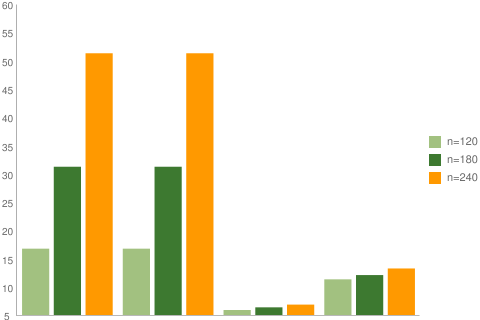
\includegraphics[width=120mm]{graph-onethread}

This is a graph of each program's performance using only one thread. Except for $nbody2$ which actually did show a bit improvement using two threads instead of one for $n=180$ and $n=240$ and slightly for three threads with $n=240$, adding additional threads seem to show no significant improvement.

\subsection{Explanation}

The $n\ log\ n$ benefits are crucial to be able to simulate more than 10000 nodes in realtime. The performance impact on larger instances (1000+) is huge. The $n=240$ instance is still quick enough to simultate in realtime with the naive sequential $n^2$ version. Even though parallelization can be useful, it can not help more than by a constant.

Larger $n$ values is where the first parallel program starts to pay off. Timing this program showed that though more cores are available they aren't used as much as desired. For these small instances no run gave anywhere near 400\% CPU time. This is believed to be because the threads aren't used long enough before sleeping to spread out on all cores. Some threads may possibly not even have time to start between barriers before the bag of tasks is finished off, as well. Leaving some threads essentially useless. This is why I did another test run with $n=10000$ to illustrate the program's parallel properties really well.

For the Barnes-Hut verions however the locking/unlocking really takes out all the fun. Profiling showed that most of the cpu time was spent locking/unlocking mutex variables (for updating node mass centers). This is why nbody3 and nbody4 show so large differences with both using the same number of processes. As moving each body requires locking each node it's in, moving $n$ bodies will require way more than locking/unlocking $n$ locks.

The locking is done per-node in the octree to update mass centers properly and not have race conditions doing so. For very large instances there's some gain, but nowhere enough to come near $nbody3$, this locking is simply too heavy for realistic instances. This might be possible to counteract with larger node sizes (less locks), but that would counter the $n\ log\ n$ properties given by the Barnes-Hut method.

\section{Conclusion}

It's been useful to parallelize the naive version, but the real benefits came from optimizing the problem using the Barnes-Hut method. Optimization is crucial to be able to run larger instances and I'd say parallelization is benefitial rather than crucial. In small instances however, this parallelization gets in the way rather than help.

It's been very interesting as well to parallelize such a fairly complex data structure as well. There are a lot of issues where synchronization errors and deadlocks can occur if not done properly.
§
As a side note the graphical interface proved really useful to understand how the simulation was working and if it seemed to be done correctly as well.

The most important thing I've learned however is how improper usage of mutex variables can break the benefits from parallelizing a program if done improperly. It's also possible that waiting for mutexes or condition variables possibly messes with the operating system's ability to distribute threads between CPU cores.

\subsection{Outlines for a better program}

What really breaks this implementation (4th, Barnes-Hut parallel program) is that every node can be touched by every thread at any time. That means that every node in the octree needs a lock. Workloads are done by splitting the body list. These bodies could be placed anywhere, meaning that bodies inside a task isn't usually anywhere near the others.

Instead, to avoid this huge locking issue, I propose that the main node is split twice, giving 64 smaller nodes. Have each of these 64 nodes be a workload. That means moving units inside this node or any of those subnodes doesn't require any locking. Finally the higher-level nodes would have their mass center and total mass updated by locking. This would however only require a few locks and wouldn't nearly hurt impact anywhere near as much.

The problem with this proposed implementation is when bodies moves outside their task node volume. Thus I propose an additional step to the adding-velocities part. When moving bodies are moved and have to be moved outside their task node volume, it gets added to a list of nodes that have to be moved from its task node. After the regular add-velocity step, there would be a step using locks to move these around. As these ``conflicting'' bodies are significantly less than the total amount of bodies, this step shouldn't have too much impact on the total performance.

By splitting tasks this way locks (and more importantly locking) is drastically reduced. This should improve performance greatly and give a performance closer to the non-parallel version of the program using only one thread as well as well improved performance with more threads.

\end{document}

